\documentclass[11pt]{article}
\PassOptionsToPackage{hyphens}{url}
\usepackage{certmachine}
\usepackage{graphicx}
%% generated by tools/paper-numbers/register.js from the records named in its header — do not edit (git be82e126bc6b)
\newcommand{\RepoCommit}{be82e126bc6b}
\newcommand{\RegDate}{2026-10-06}
\newcommand{\RegGit}{a310e6e}
\newcommand{\RegRows}{132}
\newcommand{\RegDecided}{131}
\newcommand{\RegPending}{1}
\newcommand{\RegSubmitted}{0}
\newcommand{\RegSources}{25}
\newcommand{\RegPages}{22}
\newcommand{\RegKinds}{14}
\newcommand{\RegKindsUsed}{11}
\newcommand{\VCertified}{107}
\newcommand{\VPartial}{9}
\newcommand{\VRefuted}{2}
\newcommand{\VMixed}{5}
\newcommand{\VRepaired}{6}
\newcommand{\VNeedsData}{2}
\newcommand{\VQueued}{1}
\newcommand{\RegHolds}{107}
\newcommand{\RegDefects}{24}
\newcommand{\RegHoldsPct}{82\%}
\newcommand{\RegTheorems}{109}
\newcommand{\AiRows}{107}
\newcommand{\AiRowsDefects}{17}
\newcommand{\OtherRows}{24}
\newcommand{\OtherRowsDefects}{7}
\newcommand{\KindRows}{none & the claim holds as printed & 108 & 359 \\
narrower scope & decided only in a narrower scope than printed; the rest is out of reach, not wrong & 8 & 8 \\
float printed as exact & a floating-point result printed as the exact quantity & 1 & 1 \\
sign slip & a sign wrong in a printed constant & 1 & 1 \\
arithmetic slip & a printed arithmetic step that does not hold & 2 & 27 \\
tolerance witness & a witness only within a numerical tolerance; the printed value is the tolerance's & 5 & 5 \\
not the optimum & printed as an optimum, but not the one the definition names (a stop short of it, or a local one) & 1 & 1 \\
wrong quantity & the printed number is a correct answer to a different question & 1 & 1 \\
not from the published data & the printed number is not what the published data give, and the arithmetic is not why & 1 & 2 \\
outside support & the printed model gives observed data zero density & 0 & 0 \\
clause missing from formal statement & a clause the prose claims is absent from the formal statement that is proved & 0 & 0 \\
data not public & the data behind the claim are not public, so no one outside can decide it & 2 & 2 \\
depends on reading & the claim holds under one of two definitions its own text gives, and not under the other & 1 & 1 \\
checker wider than definition & the checker that accepted the claim admits what the definition it encodes excludes & 1 & 1 \\}
\newcommand{\KNone}{108}
\newcommand{\KNarrower}{8}
\newcommand{\KFloat}{1}
\newcommand{\KSign}{1}
\newcommand{\KArith}{2}
\newcommand{\KTolerance}{5}
\newcommand{\KNotOptimum}{1}
\newcommand{\KWrongQuantity}{1}
\newcommand{\KNotFromData}{1}
\newcommand{\KOutsideSupport}{0}
\newcommand{\KClause}{0}
\newcommand{\KDataNotPublic}{2}
\newcommand{\KReading}{1}
\newcommand{\KChecker}{1}
\newcommand{\KTopDefect}{narrower scope}
\newcommand{\KTopDefectRows}{8}
\newcommand{\RegAggregates}{5}
\newcommand{\AggItems}{283}
\newcommand{\AggRows}{the published Ramanujan Machine result sheets, 52 printed rows & \textsc{mixed} & 51 none, 1 sign slip \\
the exceedance counts printed for the environmental-contour benchmark's 150 contours & \textsc{mixed} & 174 none, 2 not from the published data \\
the worked solutions of GSM8K's 8,792 test and train keys & \textsc{mixed} & 26 arithmetic slip \\
the time-horizon coefficients and 50\% horizons METR prints for 23 models & \textsc{mixed} & 22 none, 1 not the optimum \\
the 15 Hs marginal fits the benchmark teams printed for buoys A, B and C & \textsc{mixed} & 5 none, 1 wrong quantity \\}
\newcommand{\MonthRows}{August 2026 & 18 & 15 & 1 & 1 & 1 & 0 & 0 & 0 & 3 \\
September 2026 & 69 & 48 & 8 & 1 & 4 & 5 & 2 & 1 & 20 \\
October 2026 & 45 & 44 & 0 & 0 & 0 & 1 & 0 & 0 & 1 \\}
\newcommand{\MonthAugRows}{18}
\newcommand{\MonthSepRows}{69}
\newcommand{\MonthSepDecided}{68}
\newcommand{\MonthOctRows}{45}
\newcommand{\RegFirstDate}{2026-08-25}
\newcommand{\RegLastDate}{2026-10-05}
\newcommand{\RegDays}{13}
\newcommand{\McRegistered}{2026-10-02}
\newcommand{\McCount}{100}
\newcommand{\McRows}{44}
\newcommand{\McSources}{5}
\newcommand{\McPools}{10}
\newcommand{\RegBiggestDayAugSep}{2026-09-29}
\newcommand{\RegBiggestDayAugSepRows}{33}
\newcommand{\SourceRows}{Erd\H{o}s \#852, the constant $C^*$ & a problem-thread post, frontier-model help & 1 & 0 & 0 & 1 & 0 & 0 & 0 & 0 & 2026-08-25 \\
matrix-multiplication schemes & Strassen, AlphaTensor, AlphaEvolve & 10 & 10 & 0 & 0 & 0 & 0 & 0 & 0 & 2026-08-25 \\
Ramanujan Machine result sheets & the Ramanujan Machine project & 1 & 0 & 0 & 0 & 1 & 0 & 0 & 0 & 2026-08-25 \\
six AI-assisted manuscripts, lane audit & manuscripts produced with frontier-model help & 6 & 5 & 1 & 0 & 0 & 0 & 0 & 0 & 2026-08-30 \\
kissing configurations in $\mathbb{R}^{11}$ & AlphaEvolve, EinsteinArena, the Station, classical & 11 & 10 & 0 & 0 & 0 & 0 & 0 & 1 & 2026-09-03 \\
EinsteinArena state-of-the-art table & AlphaEvolve, TTT-Discover, Together AI agents, Haugland & 20 & 16 & 0 & 0 & 0 & 4 & 0 & 0 & 2026-09-08 \\
environmental-contour benchmark counts & the benchmark's teams & 1 & 0 & 0 & 0 & 1 & 0 & 0 & 0 & 2026-09-15 \\
GSM8K answer keys & GSM8K & 1 & 0 & 0 & 0 & 1 & 0 & 0 & 0 & 2026-09-21 \\
METR time-horizon fits & METR & 1 & 0 & 0 & 0 & 1 & 0 & 0 & 0 & 2026-09-22 \\
printed $H_s$ marginal fits & the benchmark's teams & 1 & 0 & 0 & 0 & 1 & 0 & 0 & 0 & 2026-09-27 \\
a printed design table & Bhaskaran et al. & 1 & 0 & 0 & 0 & 0 & 0 & 1 & 0 & 2026-09-28 \\
an AI counterexample library & Sra; GPT, Codex and Claude models & 14 & 9 & 5 & 0 & 0 & 0 & 0 & 0 & 2026-09-29 \\
registry asterisk C71 & Numaro & 1 & 1 & 0 & 0 & 0 & 0 & 0 & 0 & 2026-09-29 \\
GNNW's unverified iteration & ChatGPT 5.6 Sol, printed by Gupta et al. & 1 & 1 & 0 & 0 & 0 & 0 & 0 & 0 & 2026-09-29 \\
HorizonMath credited discoveries & GPT-5.4 and GPT-5.6 models & 3 & 1 & 0 & 1 & 0 & 0 & 1 & 0 & 2026-09-29 \\
polynomial maps, two 2026 papers & Gao with Claude; Casta\~neda et al. & 8 & 7 & 1 & 0 & 0 & 0 & 0 & 0 & 2026-09-29 \\
registry asterisks C3b, C3c & Mosaic Intelligence, Y.\ Lin & 3 & 3 & 0 & 0 & 0 & 0 & 0 & 0 & 2026-09-29 \\
registry asterisk C84b & Althoefer with ChatGPT & 1 & 0 & 0 & 0 & 0 & 1 & 0 & 0 & 2026-09-29 \\
registry asterisk C42 & Griego; R\"ohrig with Codex & 2 & 0 & 2 & 0 & 0 & 0 & 0 & 0 & 2026-09-29 \\
AlphaEvolve notebook, pre-registered & AlphaEvolve & 15 & 15 & 0 & 0 & 0 & 0 & 0 & 0 & 2026-10-04 \\
AlphaTensor over $\mathbb{F}_2$, pre-registered & AlphaTensor & 8 & 8 & 0 & 0 & 0 & 0 & 0 & 0 & 2026-10-04 \\
AlphaTensor, standard arithmetic, pre-registered & AlphaTensor & 12 & 12 & 0 & 0 & 0 & 0 & 0 & 0 & 2026-10-04 \\
EinsteinArena bests, pre-registered & EinsteinArena agents & 8 & 7 & 0 & 0 & 0 & 1 & 0 & 0 & 2026-10-05 \\
the Station, pre-registered & the Station's agents & 1 & 1 & 0 & 0 & 0 & 0 & 0 & 0 & 2026-10-05 \\
Navier--Stokes Lean certificate & OpenAI & 1 & 1 & 0 & 0 & 0 & 0 & 0 & 0 & 2026-10-05 \\}
\newcommand{\DateRows}{2026-08-25 & 11 & Erd\H{o}s \#852, the constant $C^*$; Ramanujan Machine result sheets; matrix-multiplication schemes \\
2026-08-26 & 1 & matrix-multiplication schemes \\
2026-08-30 & 6 & six AI-assisted manuscripts, lane audit \\
2026-09-03 & 11 & kissing configurations in $\mathbb{R}^{11}$ \\
2026-09-08 & 20 & EinsteinArena state-of-the-art table \\
2026-09-15 & 1 & environmental-contour benchmark counts \\
2026-09-21 & 1 & GSM8K answer keys \\
2026-09-22 & 1 & METR time-horizon fits \\
2026-09-27 & 1 & printed $H_s$ marginal fits \\
2026-09-28 & 1 & a printed design table \\
2026-09-29 & 33 & registry asterisks C3b, C3c; registry asterisk C71; registry asterisk C84b; registry asterisk C42; an AI counterexample library; HorizonMath credited discoveries; GNNW's unverified iteration; polynomial maps, two 2026 papers \\
2026-10-04 & 35 & AlphaEvolve notebook, pre-registered; AlphaTensor over $\mathbb{F}_2$, pre-registered; AlphaTensor, standard arithmetic, pre-registered \\
2026-10-05 & 10 & Navier--Stokes Lean certificate; EinsteinArena bests, pre-registered; the Station, pre-registered \\}
\newcommand{\RegBiggestDay}{2026-10-04}
\newcommand{\RegBiggestDayRows}{35}
\newcommand{\RegWhat}{Externally published mathematical claims this machine has decided, one row per claim, each derived from the record that decided it. The verdicts are the instrument's, not a summary: CERTIFIED and REFUTED are theorems, PARTIAL names the fragment that was reached, NEEDS DATA measures the claimant rather than the claim, MIXED means the row is an aggregate whose record holds both, and REPAIRED means the claim as printed is refuted and an object next to it is certified. Each row names its defect kind from one closed vocabulary (kindsDefined); an aggregate row counts them. recordedOn is the first commit whose deciding record held the row.}
\newcommand{\RegScope}{claims that come down to finitely many exact arithmetic facts --- exhibit a witness, verify an identity, bound a quantity, decide a constant. Everything else is REFUSED as out of scope rather than guessed at.}
\newcommand{\CstarPublished}{0.0752403861777}
\newcommand{\CstarLo}{0.0752403861783092455893}
\newcommand{\CstarHi}{0.0752403861783095651674}
\newcommand{\CstarDefinition}{(1/2)(prod over primes p>=3 of (1 + 1/(p-1)\textasciicircum{}3) - 1)}
\newcommand{\CstarPrimes}{1{,}857{,}858}
\newcommand{\CstarPrimeBound}{30{,}000{,}000}
\newcommand{\CstarBits}{192}
\newcommand{\CstarLimit}{400{,}000}
\newcommand{\CstarInequality}{5\cdot (N-D)\cdot 10^{12} > 752403861778\cdot D}
\newcommand{\CstarWindowNum}{752403861778}
\newcommand{\CstarWindowDen}{13}
\newcommand{\CstarThreshold}{208{,}064}
\newcommand{\CstarVanish}{87\%}
\newcommand{\CstarPlace}{12}
\newcommand{\CstarSig}{11}
\newcommand{\CstarPublishedDigits}{12}
\newcommand{\CstarThreadDate}{2026-04-24}
\newcommand{\CzeroPublished}{1.32322827686395}
\newcommand{\CzeroDigits}{61}
\newcommand{\CstarVerifier}{tools/verify\_erdos852.py}
\newcommand{\SpClaim}{C84b <= 1.999281 (c >= 0.000719)}
\newcommand{\SpRepairedTo}{C84b <= 1.9993 (c >= 0.0007, the note's own theorem)}
\newcommand{\SpCeiling}{0.0007150507}
\newcommand{\SpAtNote}{0.0007062455}
\newcommand{\SpQuotedC}{0.000719}
\newcommand{\SpTheoremC}{0.0007}
\newcommand{\SpNoteDate}{2026-05-28}
\newcommand{\SpNoteAuthor}{Ingo Althoefer}
\newcommand{\SpNoteTitle}{Improved constant for [BSSZ2026]}
\newcommand{\SpRegistryCommit}{2c1968cd}
\newcommand{\SpChecks}{7}
\newcommand{\SpCheckRows}{1 & \texttt{f(1.371966384) <= 103 (the note: about 101.956)} & \texttt{[101.9560758327, 101.9560758327]} \\
2 & \texttt{515/Y = 515/1415 < 0.364} & --- \\
3 & \texttt{M1 e\textasciicircum{}Y/(X Y\textasciicircum{}2) + M2/(X\textasciicircum{}2 Y\textasciicircum{}2) < 0.136 (and so < 0.364)} & \texttt{0.1352394769} \\
4 & \texttt{log|A|/d < L < 1432} & \texttt{1431.1139757} \\
5 & \texttt{-log(0.364) > 0.0007 * 1432 = 1.0024: c = 0.0007 holds} & \texttt{1.01060141} \\
6 & \texttt{inf over s > 1 of f(s) >= 101.9 (a sweep of [1.01, 2.9] by 0.001, of [1.2, 1.6] by 0.0001; below, zeta > 100; above, the power dominates)} & \texttt{smallest endpoint bound 101.927484 at s = 1.372} \\
7 & \texttt{for every s > 1, X and Y, the chain gives c <= 0.0007150 < 0.000719} & \texttt{the maximum near Y = 1399.0} \\}
\newcommand{\SpClaimant}{I. Althoefer with ChatGPT 5.5 (the note, 28 May 2026), as the registry quotes it}
\newcommand{\DtAreas}{5}
\newcommand{\DtDecided}{20}
\newcommand{\DtOff}{19}
\newcommand{\DtOutside}{1}
\newcommand{\DtCitation}{Bhaskaran, S. K., Verma, A. S., Goupee, A. J., Bhattacharya, S., Nejad, A. R., Shi, W. (2023). Comparison of Extreme Wind and Waves Using Different Statistical Methods in 40 Offshore Wind Energy Lease Areas Worldwide. Energies 16(19), 6935.}
\newcommand{\DtDoi}{10.3390/en16196935}
\newcommand{\DtPrivate}{WaveClimate, 1992--2022}
\newcommand{\DtPublic}{Ifremer GLOBMULTI\_\allowbreak{}ERA5\_\allowbreak{}GLOBCUR\_\allowbreak{}01, 1993--2024, CC BY-SA 4.0}
\newcommand{\DtKmMin}{31}
\newcommand{\DtKmMax}{61}
\newcommand{\DtYears}{32}
\newcommand{\DtLevelRows}{UY01 & Gumbel, least squares & 10.09 & 8.38 & +1.71 \\
UY01 & Gumbel, max.\ likelihood & 9.48 & 8.38 & +1.10 \\
UY01 & Gumbel, moments & 9.70 & 8.38 & +1.32 \\
UY01 & GEV, max.\ likelihood & 9.01 & 9.61 & $-$0.59 \\
Projeto Açu & Gumbel, least squares & 5.55 & 3.21 & +2.34 \\
Projeto Açu & Gumbel, max.\ likelihood & 5.46 & 3.21 & +2.24 \\
Projeto Açu & Gumbel, moments & 5.33 & 3.21 & +2.12 \\
Projeto Açu & GEV, max.\ likelihood & 6.36 & 3.22 & +3.14 \\
Farol wind & Gumbel, least squares & 7.84 & 5.86 & +1.99 \\
Farol wind & Gumbel, max.\ likelihood & 7.49 & 5.86 & +1.64 \\
Farol wind & Gumbel, moments & 7.54 & 5.86 & +1.68 \\
Farol wind & GEV, max.\ likelihood & 7.40 & 5.76 & +1.65 \\
Sopros do RJ & Gumbel, least squares & 4.06 & 5.47 & $-$1.41 \\
Sopros do RJ & Gumbel, max.\ likelihood & 3.98 & 5.47 & $-$1.49 \\
Sopros do RJ & Gumbel, moments & 3.94 & 5.47 & $-$1.54 \\
Sopros do RJ & GEV, max.\ likelihood & 4.14 & 5.04 & $-$0.90 \\
Projeto Ubu & Gumbel, least squares & 3.20 & 4.93 & $-$1.73 \\
Projeto Ubu & Gumbel, max.\ likelihood & 3.03 & 4.93 & $-$1.90 \\
Projeto Ubu & Gumbel, moments & 3.07 & 4.93 & $-$1.85 \\
Projeto Ubu & GEV, max.\ likelihood & 2.83 & 4.86 & $-$2.03 \\}
\newcommand{\DtMatrixRows}{UY01 & 10.09 / 8.38 & 9.48 / 8.38 & 9.70 / 8.38 & 9.01 / 9.61 \\
Projeto Açu & 5.55 / 3.21 & 5.46 / 3.21 & 5.33 / 3.21 & 6.36 / 3.22 \\
Farol wind & 7.84 / 5.86 & 7.49 / 5.86 & 7.54 / 5.86 & 7.40 / 5.76 \\
Sopros do RJ & 4.06 / 5.47 & 3.98 / 5.47 & 3.94 / 5.47 & 4.14 / 5.04 \\
Projeto Ubu & 3.20 / 4.93 & 3.03 / 4.93 & 3.07 / 4.93 & 2.83 / 4.86 \\}
\newcommand{\DtMaxGap}{3.14}
\newcommand{\DtMinGap}{0.59}
\newcommand{\KissNeedsFrom}{2026-09-03}
\newcommand{\KissBytes}{2026-09-07}
\newcommand{\KissDays}{4}
\newcommand{\KissContacts}{19{,}704}
\newcommand{\KissMs}{130}
\newcommand{\KissN}{604}
\newcommand{\KissRows}{11}
\newcommand{\KissCertified}{10}
\newcommand{\KissQueued}{1}
\newcommand{\HmPoints}{201}
\newcommand{\HmOutside}{56}
\newcommand{\HmNotPlaced}{128}
\newcommand{\HmNotRefuted}{17}
\newcommand{\HmC}{3.6960839126}
\newcommand{\HmGnnw}{3.7992}
\newcommand{\HmGapE}{13/2000}
\newcommand{\HmGapP}{11981/500000}
\newcommand{\HmGap}{0.00130}
\newcommand{\HmXone}{0.22745}
\newcommand{\HmYone}{0.9988}
\newcommand{\HmEU}{0.26292}
\newcommand{\HmCheckerLine}{299}
\newcommand{\HmKakeyaNum}{6008623}
\newcommand{\HmKakeyaDen}{55{,}050{,}240}
\newcommand{\HmKakeyaDec}{0.1091479891}
\newcommand{\HmKakeyaPieces}{4{,}033}
\newcommand{\HmCommit}{4ef0b61a}
\newcommand{\EaRows}{20}
\newcommand{\EaWitnessed}{16}
\newcommand{\EaRepaired}{4}
\newcommand{\EaProblems}{8}
\newcommand{\EaCommit}{c388c6f7}
\newcommand{\EaCirclesDeficit}{$8.67\times10^{-11}$}
\newcommand{\EaCirclesOverlaps}{44}
\newcommand{\EaCirclesPrinted}{2.3658323759}
\newcommand{\EaCirclesExact}{2.3658323758}
\newcommand{\EaOverlapRepairs}{3}
\newcommand{\EaOverlapMiss}{$1.48\times10^{-14}$}
\newcommand{\EaOverlapDeltaMax}{$8.32\times10^{-18}$}
\newcommand{\EaCirclesPublished}{2026-04-02}
\newcommand{\EaCirclesSlackDropped}{2026-08-24}
\newcommand{\EaRuleAsOf}{2026-10-06}
\newcommand{\AiLanes}{6}
\newcommand{\AiConfirmed}{5}
\newcommand{\AiPartial}{1}
\newcommand{\AiRefuted}{0}
\newcommand{\AiChecks}{92}
\newcommand{\AiChecksFrom}{4}
\newcommand{\AiMutations}{21}
\newcommand{\AiSeconds}{4.6}
\newcommand{\LaneRows}{Maxwell's point-charge bound & \textsc{certified} & at $\varepsilon$ = 1/6 only & 17 & 3 \\
The Korenblum constant & \textsc{certified} & the numerical criterion & 15 & 4 \\
Erdős Problem \#1038 & \textsc{certified} & the computational fragment & 22 & 4 \\
Ran--Teng Conjecture 20 & \textsc{partial} & machine-checkable fragment only & 38 & 5 \\
The Mathieu property for Lie groups & \textsc{certified} & supporting identities only & --- & 3 \\
The rank-two Poisson conjecture & \textsc{certified} & the explicit counterexample & --- & 2 \\}
\newcommand{\RmCertified}{52}
\newcommand{\RmPrinted}{51}
\newcommand{\RmSurvive}{50}
\newcommand{\RmRefuted}{1}
\newcommand{\RmCorrections}{1}
\newcommand{\RmRegisterSays}{the published Ramanujan Machine result sheets, 52 printed rows; 51 rows survive their certified enclosure, 1 refuted exactly}
\newcommand{\RmRegisterPrinted}{52}
\newcommand{\RmErratum}{counts}
\newcommand{\LoopRefused}{73}
\newcommand{\LoopDecided}{16{,}951}
\newcommand{\LoopFamilies}{11}
\newcommand{\LoopWhere}{chowla-cosine, keller-fibers}
\newcommand{\GsItems}{8{,}792}
\newcommand{\GsTest}{1{,}319}
\newcommand{\GsTrain}{7{,}473}
\newcommand{\GsAnnotations}{27{,}998}
\newcommand{\GsAnnotExact}{27{,}996}
\newcommand{\GsAnnotRefused}{2}
\newcommand{\GsWrong}{26}
\newcommand{\GsWrongTest}{2}
\newcommand{\GsWrongTrain}{24}
\newcommand{\EcContours}{150}
\newcommand{\EcComparisons}{176}
\newcommand{\EcAgree}{174}
\newcommand{\EcExact}{173}
\newcommand{\EcDisagree}{2}
\newcommand{\EcNotSimple}{30}
\newcommand{\MeFits}{44}
\newcommand{\MeLive}{23}
\newcommand{\MeReproduced}{22}
\newcommand{\MeScope}{44 of 44 fits certified; the printed coefficients are the rounding of the certified optimum for 22 of 23; the printed 50\% horizons lie inside the enclosure for 0 of 23 (an optimiser's tolerance, all inside METR's own bootstrap interval)}
\newcommand{\HsPrinted}{15}
\newcommand{\HsScope}{5 reproduce a certified maximum-likelihood fit; 1 printed as Hs reproduce the certified fit of Tz; 0 stated as maximum likelihood are off its maximum; 3 use another estimator (least squares) and are not decided here; 6 are not decidable at the printed precision}
\newcommand{\HsOk}{5}
\newcommand{\HsTz}{1}
\newcommand{\MmRows}{10}
\newcommand{\MmAlphaTensor}{7}
\newcommand{\MmAlphaEvolve}{1}
\newcommand{\MmCalibration}{2}
\newcommand{\MmCharTwo}{2}
\newcommand{\PmRows}{8}
\newcommand{\PmCertified}{7}
\newcommand{\PmPartial}{1}
\newcommand{\CxRows}{14}
\newcommand{\CxCertified}{9}
\newcommand{\CxPartial}{5}
\newcommand{\CxCommit}{dbf67374}
\newcommand{\OcRows}{7}
\newcommand{\OcAsterisks}{5}
\newcommand{\OcRegistryCommit}{2c1968cd}
\newcommand{\OcStarNote}{''Bounds for which the level of available verification is currently at minimal levels will be marked with an asterisk''}
\newcommand{\GnC}{3.78232877553}
\newcommand{\GnPrintedIs}{its rounding}
\newcommand{\NsJobs}{2{,}486}
\newcommand{\NsCommit}{8937a8f4}
\newcommand{\NsHeadCommit}{f9e8bc5b}
\newcommand{\NsHeadDate}{2026-09-10}
\newcommand{\NsRecorded}{2026-10-05}
\newcommand{\NsPriorRecorded}{2026-09-09}
\newcommand{\EvRows}{364}
\newcommand{\EvCertified}{115}
\newcommand{\EvRejected}{147}
\newcommand{\EvMalformed}{39}
\newcommand{\EvDeclined}{23}
\newcommand{\EvBudget}{40}
\newcommand{\EvClaims}{301}
\newcommand{\EvRefusalRate}{13.0\%}
\newcommand{\EvModels}{3}
\newcommand{\RefusalRows}{\textsc{refused} & the engine loop (the instrument declined to decide an object it enumerated) & 73 & 16{,}951 & objects certified \\
\textsc{refused} & the matrix-multiplication eval board (a submitted reply carried no parseable proposal) & 39 & 301 & claims submitted \\
\textsc{needs data} & the kissing ledger (decidable, but the claimant had published no bytes) & 0 & 11 & ledger rows \\
\textsc{open} & the Erd\H{o}s \#1038 supremum campaign (a degree attempted, budget exhausted, recorded) & 1 & 7 & degrees attempted \\
\textsc{open} & the $\lambda(6)$ campaign (a family still computing, published as unfinished) & 1 & 10 & families in the worklist \\
\textsc{undecided} & the two-population regime map (a swept cell whose box did not close) & 9{,}915 & 21{,}567 & cells swept \\
\textsc{undecided} & the one-population regime map & 8{,}086 & 19{,}800 & cells swept \\
\textsc{scope} & the six-lane audit (a lane that reached a fragment and says which) & 6 & 6 & lanes audited \\}
\newcommand{\RefKinds}{5}
\newcommand{\RefUndecided}{18{,}001}
\newcommand{\RefCells}{41{,}367}
\newcommand{\RefUndecidedPct}{43.5\%}
\newcommand{\SubFailedDegree}{deg9}
\newcommand{\LamClosed}{9}
\newcommand{\LamWorklist}{10}
\newcommand{\LfBox}{30}
\newcommand{\LfSets}{25{,}819}
\newcommand{\LfFinite}{423}
\newcommand{\LfRefuters}{0}
\newcommand{\LfDate}{2026-09-01}
\newcommand{\LfClosed}{2{,}231}
\newcommand{\LfSkips}{6}
\newcommand{\LfFamilies}{9}
\newcommand{\LfGeneric}{14}
\newcommand{\LfOutsideDate}{2026-09-30}
\newcommand{\LfOutsideRepo}{rainrzk/erdos510-lambda4-audit}
\newcommand{\LfOutsideUrl}{https://github.com/rainrzk/erdos510-lambda4-audit}
\newcommand{\LfIssue}{392}
\newcommand{\LfOutsideMax}{80}
\newcommand{\LfRival}{\{2,3,4,6\}}
\newcommand{\LfRivalValue}{$-1.774$}
\newcommand{\LfFindings}{three}
\newcommand{\BugsN}{16}
\newcommand{\BugsMechanisms}{6}
\newcommand{\BugRows}{code read & 6 \\
impossible number & 3 \\
outside read & 2 \\
calibration & 2 \\
control & 2 \\
byte pin & 1 \\}
\newcommand{\BugsByCodeRead}{6}
\newcommand{\BugsByRunning}{10}
\newcommand{\CheatsN}{19}
\newcommand{\GatesN}{7}
\newcommand{\PosDate}{2026-09-03}


\theoremstyle{plain}
\newtheorem{decision}{Decision}
\theoremstyle{definition}
\newtheorem{definition}{Definition}

\title{Independent exact certification of machine-generated mathematics:\\ the first register}
\author{\cmauthor}
\date{October 2026 --- draft v0.1 for review; every number interpolated from the record; machine-derived, not peer-reviewed; author list to be agreed}

\begin{document}
\maketitle

\begin{abstract}
Mathematics now arrives from machines as exact objects with enclosures: constants, counterexamples, packings, matrix-multiplication schemes and certificates for asymptotic bounds, each validated by the checker of the group that produced it. This paper describes a method for deciding such claims independently --- in exact rational and outward-rounded interval arithmetic, with no code shared with the claimant, and with refusal as a published result --- and presents its evidence, a register of \RegRows{} published claims decided between \RegFirstDate{} and \RegLastDate{}: \VCertified{} certified, \VRefuted{} refuted, \VPartial{} partial, \VMixed{} mixed, \VRepaired{} repaired, \VNeedsData{} needing data the claimant has not published, and \VQueued{} queued and not counted. Every row is derived from a record that re-runs, carries the witness its verdict needs, and names what went wrong from a closed vocabulary of \RegKinds{} defect kinds. Most claims hold: \RegHolds{} of the \RegDecided{} decided rows name nothing wrong. The defects that do appear are of the verifier's kind rather than the mathematician's --- a floating-point product printed as an exact constant, witnesses that hold only within a verifier's tolerance, a checker that accepts what its own definition excludes --- and one row keeps as its history a clause present in a paper's theorem and absent from its formal statement, until the claimant's next commit proved it. The novelty claimed is the decision grammar (verdict, witness, refusal as a result) and the public re-runnable record, not interval arithmetic. The method runs both ways: a theorem of this laboratory re-certified by an outside audit with no shared code is recorded like any other row.
\end{abstract}

\section{Introduction}

\subsection{Where the claims come from}

In 2025 and 2026 a large part of newly announced mathematics has been produced, in whole or in part, by machines, and has arrived in a form that is new: not a proof to be read but an object to be checked. AlphaEvolve \cite{Novikov25,Georgiev25} publishes packings, step functions and polynomials as coordinate files; AlphaTensor \cite{Fawzi22} publishes tensor decompositions; agent platforms such as EinsteinArena \cite{Bianchi26} and the Station \cite{Chung26} publish kissing configurations and tables of constructions scored by their own verifiers; test-time discovery systems \cite{Yuksekgonul26} publish step functions with six hundred steps. A benchmark, HorizonMath \cite{Wang26}, credits frontier models with discoveries and accepts a closed form on a twenty-digit numerical match while saying that this is not a proof. A library of counterexamples found by language models \cite{Sra26} ships a certificate per case. A registry of optimisation constants marks bounds whose verification is ``at minimal levels'' with an asterisk \cite{OptReg}. A paper on diagonal Ramsey numbers prints, after a remark, an improvement proposed by a chat model and labels it preliminary and unverified \cite{GNNW24}. Counterexamples to the Jacobian conjecture in dimension three \cite{Gao26} and to the weak Markus--Yamabe conjecture in dimension fourteen \cite{CHV26} are polynomial maps whose claimed properties are identities. On a problem thread a model-produced constant was posted to thirteen decimals with no error bound \cite{ErdosProblems}.

What these have in common is that each claim comes down to finitely many exact arithmetic facts, and that each was validated, if at all, by the checker of the group that produced it. The tools to decide such facts without error are old: interval arithmetic with outward rounding \cite{MKC09,Tucker11}, exact rational arithmetic, and the discipline of computer-assisted proof that reached its public standard with the formal Kepler proof \cite{Hales17}. What did not exist was an independent party applying them to the stream, with a grammar for the outcomes and a public record of every decision, including the ones that went nowhere. A verifier that only ever passes or fails is a scorer, and scorers are what the stream is full of; an audit of reward verifiers in reinforcement learning found a reference numeric verifier that accepts every off-by-one answer above ten thousand \cite{Xin26}. The missing third outcome --- this claim cannot be decided here, and here is why --- is the one a motivated party never builds.

\subsection{What this paper is}

This is the method paper of a project whose position, adopted on \PosDate{} and held since \cite{Positioning}, is one sentence: \emph{independent exact certification of machine-generated mathematics --- exact arithmetic, no code shared with the claimant, refusal as a verdict.} The paper states the decision grammar (\S\ref{sec:grammar}), the discipline that keeps it honest (\S\ref{sec:discipline}), and the register that is its evidence (\S\ref{sec:register}): \RegRows{} rows derived from \RegSources{} records, each decided by an instrument written from the published statement and the published bytes, never from the claimant's code. Three rows are worked in a page each (\S\ref{sec:examples}): a refutation with its witness, a repair, and a refusal with the one thing that would decide it. Section~\ref{sec:measures} reads the register as a measurement of what goes wrong in machine-generated mathematics; \S\ref{sec:recert} records the direction the method must also run in, a theorem of this laboratory re-certified by an outside audit with no shared code. Sections~\ref{sec:notclaimed} and \ref{sec:limits} say what is not claimed and where the method stops.

The project's own mathematical records --- the value of $\lambda(4)$ in Chowla's cosine problem \cite{Lambda4}, the dimension-eleven kissing ledger \cite{Kissing}, the explicit sum-distinct sets below Bohman's constant \cite{Erdos1} --- are cited as records and not restated. The novelty line is deliberately narrow: not interval arithmetic, which is standard, but the grammar of verdict, witness and refusal, and a register every row of which re-runs from a public record.

\section{Statement of results}\label{sec:results}

The results are of three kinds, and the paper keeps them apart: counts, which are facts about a record; theorems, which the record proves; and decisions, which are the instrument's outcomes stated as such.

\begin{proposition}[the register, as recorded]\label{prop:register}
As of \RegDate{} (git \RegGit{}), the register of \S\ref{sec:register} holds \RegRows{} rows, each derived from one of \RegSources{} records and dated by the first commit whose record held it. \RegDecided{} are decided and \RegPending{} is queued: \VCertified{} \textsc{certified}, \VRefuted{} \textsc{refuted}, \VPartial{} \textsc{partial}, \VMixed{} \textsc{mixed}, \VRepaired{} \textsc{repaired}, \VNeedsData{} \textsc{needs data}. Every row is self-initiated and \RegSubmitted{} were submitted by others. \RegHolds{} decided rows name no defect; \RegDefects{} name one of \RegKindsUsed{} kinds from a closed vocabulary of \RegKinds{}.
\end{proposition}

\begin{theorem}[a published constant, refuted]\label{thm:cstar}
Let $C^*=\tfrac12\bigl(\prod_{p\ge3}(1+1/(p-1)^3)-1\bigr)$, the product over odd primes. Then
\[
\CstarLo{} \;<\; C^* \;<\; \CstarHi{},
\]
and the value $\CstarPublished$ published for $C^*$ on the Erd\H{o}s problem \#852 thread on \CstarThreadDate{} is not $C^*$ under either a truncation or a rounding reading: it parts from the enclosure at its \CstarPlace{}th decimal place (the \CstarSig{}th significant digit). The refutation needs no tail bound: with $N/D$ the exact partial product over primes $3\le p\le\CstarLimit$, a strict lower bound for the full product, one integer inequality,
\[
\CstarInequality ,
\]
already places $(N/D-1)/2$ above the upper edge of the published window.
\end{theorem}

\begin{proposition}[a registry constant, repaired]\label{prop:repair}
Decided from the note the registry cites \cite{Althoefer26}, given that note's chain (the explicit constant of its source, its lattice-doubling lemma and its regulator bound): for every choice of the chain's parameters $s>1$, $X$ and $Y$ the exponent satisfies $c\le\SpCeiling<\SpQuotedC$, so the registry's asterisked bound $C_{84b}\le1.999281$ ($c\ge\SpQuotedC$) is out of reach of the calculation cited; the note's own theorem, $c\ge\SpTheoremC$ ($C_{84b}\le1.9993$), holds, and at the note's own parameter choice $c=\SpAtNote$.
\end{proposition}

\begin{decision}[a printed design table, refused]\label{dec:table}
The \DtDecided{} annual-maximum $H_s$ fits printed for \DtAreas{} South Atlantic lease areas \cite{Bhaskaran23} are decidable and not decided: \textsc{needs data}. They are fits to a commercial hindcast (\DtPrivate) that nobody outside can re-run. Against the nearest open-sea cells of the public hindcast the paper also names (\DtPublic), \DtKmMin{}--\DtKmMax{} km from the printed coordinates, \DtOff{} are off the certified maximum-likelihood fit and \DtOutside{} gives the record zero density --- which measures the distance between two records, not an error in the table. One file decides the row: the annual maxima the authors fitted.
\end{decision}

\begin{proposition}[a theorem of this laboratory, re-certified outside]\label{prop:recert}
The proof of the value of $\lambda(4)$ \cite{Lambda4} decides \LfClosed{} finite sets across \LfFamilies{} families (\LfSkips{} skips, all of the extremizer). On \LfOutsideDate{} an outside audit with no shared code \cite{Lambda4Audit} re-derived the cubic, the \LfGeneric{} generic collisions and the \LfFamilies{} families from the write-up, re-certified every finite case in interval arithmetic, and swept every gcd-reduced $4$-set with largest element at most \LfOutsideMax{} as a proof-independent control, finding $\{1,2,3,4\}$ deepest and the nearest rival \LfRival{} at about \LfRivalValue{}. Its \LfFindings{} documentation findings were folded into the write-up; no step broke.
\end{proposition}

\section{The grammar}\label{sec:grammar}

\begin{definition}[certified]\label{def:certified}
A claim is \emph{certified} when a finite set of exact arithmetic facts that imply it has been decided --- each in exact rational arithmetic (which decides ties) or in outward-rounded interval arithmetic (which bounds what cannot be computed exactly) --- and a certificate re-runs without this engine present and carries the input that would make it fail. ``Certified'' is used in this paper in that sense only; a result decided this way is said to be \emph{decided}, and when the facts amount to a proof, \emph{proved}.
\end{definition}

The instrument returns three verdicts and no fourth. \textsc{certified} and \textsc{refuted} are theorems about the claim as stated, each carrying a witness: for a certification, the certificate and its falsifier; for a refutation, the printed falsifying object --- an inequality, a pair outside a region, a violated equation. \textsc{refused} is what a claim receives when the instrument cannot decide it: a real outcome, published like the others, and evidence of nothing either way. A refusal is terminal. It is never retried at lower rigour, never converted to a probability, and never dropped from the record; the only path from \textsc{refused} to \textsc{certified} is a new exact argument.

The register's other words are compositions of these three, not additional verdicts, and each names which of the three it is composed of (Table~\ref{tab:grammar}). The register states it in its own header: \textsc{certified} and \textsc{refuted} are theorems, \textsc{partial} names the fragment that was reached, \textsc{needs data} measures the claimant rather than the claim, \textsc{mixed} means the row is an aggregate whose record holds both, and \textsc{repaired} means the claim as printed is refuted and an object next to it is certified.

\begin{table}[h]\centering\small
\begin{tabular}{@{}llp{0.5\linewidth}@{}}\toprule
word & composed of & the witness the row carries \\\midrule
\textsc{certified} & --- & a certificate with its falsifier; re-runs without the engine \\
\textsc{refuted} & --- & the falsifying object, printed \\
\textsc{refused} & --- & the reason, in a sentence; nothing else \\
\textsc{partial} & certified $+$ refused & which fragment certified and which core was not reached \\
\textsc{needs data} & refused, cause with the claimant & the bytes that would decide the row, named \\
\textsc{mixed} & certified $+$ refuted, one record & the counts of both, and the items refuted \\
\textsc{repaired} & refuted $+$ certified & the object as printed refuted; the object beside it certified, with its deficit \\
\textsc{queued} & not a verdict & nothing; the row is not counted as decided \\
\bottomrule\end{tabular}
\caption{The grammar. Three verdicts; four compositions, each of which says what it is made of; and one state that is not a verdict.}\label{tab:grammar}
\end{table}

Two consequences follow and are enforced rather than recommended. First, a scope sentence is load-bearing: a \textsc{certified} without the scope beside it says something the record does not, because several rows certify the computational fragment of a claim whose analytic core was never touched. Second, the kinds of refusal are never summed. The instrument declining (\textsc{refused}), the claimant having published nothing (\textsc{needs data}), a budget running out with the attempt recorded (\textsc{open}), a swept cell whose box did not close (\textsc{undecided}) and an audit stating its reach (\textsc{scope}) are five behaviours; one ``total refusals'' number would be a bigger number and a smaller fact, so the project's refusals page carries each kind with its own denominator and has no total (Table~\ref{tab:refusals}).

\section{The discipline}\label{sec:discipline}

Five rules make the grammar hold under pressure. They are stated as engineering, because each is enforced by code that refuses rather than by a sentence that advises.

\paragraph{Screens prune, never admit.} Floating point decides only what is worth certifying. Nothing a screen passes is believed; every admission is an exact decision. In the project's generation loop, the campaign runner behind its own records, a screen is required before any run to recover a planted set of known answers, so a filter that quietly drops hard cases refuses the run by name \cite{MethodsNote}.

\paragraph{Red controls must fire.} A check that has never gone red is decoration. The certificate constructor in the interval toolkit refuses to build a certificate without a falsifier --- the input that would make it fail --- and refuses a \textsc{proved} verdict with no evidence. Every battery carries deliberate forgeries that must be rejected: in the six-lane manuscript audit, \AiMutations{} mutation controls stand beside \AiChecks{} named checks and a control that stops firing refuses the page; the campaign runner ships \CheatsN{} ways to cheat its own reward signal, each caught by a named control at every build \cite{MethodsNote}. The methods note records \BugsN{} real defects this project shipped and then found: none was found by reading code; all were caught by an impossible number, a calibration, a control, a byte pin or an outside read (Table~\ref{tab:bugs}).

\paragraph{Pin the bytes.} Every transcribed claim is decided against a held byte sequence, path and sha256, re-hashed at decision time. One catalogued bug --- a row silently missing from a transcription of a published sheet --- was caught by nothing else.

\paragraph{No code shared with the claimant.} The claimant's program is never in the trust path: the decision is re-derived from the published statement and the published bytes. The precise form, adopted after a check of the unqualified phrase \cite{Positioning}, is \emph{independence from the claimant}: two of the project's own instruments reuse the project's own code across a producer/checker line, and the positioning note names both. Where an author's script was read to settle which identities a manuscript meant, the lane says so and the script was not executed.

\paragraph{Honest counting.} Every row is derived from a record; a claim with no record gets no row. An aggregate audit --- a dataset's keys, a benchmark's counts --- is one row that counts once and names its most frequent defect, because a key, a contour and a construction are not units of one another. A correction the project adds beside a refuted row is never counted among the audited corpus's rows. A queued row is not a decided row. Origin is tracked separately, and the register's submitted count stays at \RegSubmitted{} until someone sends something. Refusal kinds are never merged. Each of these rules is a line that makes a build refuse.

\begin{table}[h]\centering\small
\begin{tabular}{@{}lr@{}}\toprule
caught by & defects \\\midrule
\BugRows
reading the code & 0 \\
\bottomrule\end{tabular}
\caption{The \BugsN{} defects of the methods note \cite{MethodsNote}, by what surfaced each; parsed from the note's own catalogue, which runs \GatesN{} batteries at every build and refuses if one goes red.}\label{tab:bugs}
\end{table}

\section{The register}\label{sec:register}

\subsection{How a row is made and dated}

The register is derived, never typed. The tool that writes it reads \RegSources{} records on disk, each the output of an instrument that decided some published claim, and emits one row per claim with the claimant, the source as pinned, the verdict, the scope sentence, the defect kind, and the record and page it came from. A row names its defect kind from one closed vocabulary defined in that tool and nowhere else; a defect that fits no kind refuses the register until the vocabulary is decided on, never ``other''. The day a row entered is the first commit whose deciding record held the row's key, found with git's pickaxe on the record, so the register is a dated diff of the records rather than a log of sessions. The monthly ledger is that diff cut by month, with its first instance September 2026 \cite{Monthly}.

\subsection{By source and verdict}

Table~\ref{tab:sources} is the register grouped by the record each row was derived from, in the order the records entered. The claimant column is coarse on purpose: it says whose bytes were decided, not whose mathematics is better.

\begin{table}[htbp]\centering\footnotesize
\setlength{\tabcolsep}{3.5pt}
\resizebox{\linewidth}{!}{%
\begin{tabular}{@{}p{1.75in}p{1.95in}rrrrrrrrl@{}}\toprule
record & whose bytes & rows & \textsc{cert} & \textsc{part} & \textsc{ref} & \textsc{mix} & \textsc{rep} & \textsc{nd} & \textsc{q} & entered \\\midrule
\SourceRows
\bottomrule\end{tabular}}
\caption{The register by source. \RegRows{} rows from \RegSources{} records on \RegPages{} pages; a row counts once, an aggregate row is one audit. The entered column is the first commit whose record held the source's first row.}\label{tab:sources}
\end{table}

Three things in the table deserve a sentence each. The \MmRows{} rows of the matrix-multiplication record are \MmCalibration{} calibrations (Strassen's scheme \cite{Strassen69} and its exact Kronecker square), \MmAlphaTensor{} AlphaTensor schemes and \MmAlphaEvolve{} AlphaEvolve scheme; \MmCharTwo{} of them are certified over $\mathbb{F}_2$ and refuted over $\mathbb{Q}$, which is not a defect but the content of the claim, and the scope sentence says so. The \EaRows{} EinsteinArena table rows decide every construction that platform's state-of-the-art table publishes, across \EaProblems{} problems and including one human construction \cite{Haugland16}, from the bytes as the decimals they print: \EaWitnessed{} are exact witnesses of the value stated and \EaRepaired{} are witnesses only within a verifier's tolerance (the platform's $10^{-9}$ on one circle packing, in force when it was published and removed since; the repository notebook's $10^{-6}$ on three step-function sums), each repaired to an exact witness with its deficit printed. The one \textsc{queued} row of the register is the 2022 kissing record the machine ladder started from \cite{Ganzhinov22}, whose bytes have not yet been pulled. The \CxRows{} rows of the counterexample library \cite{Sra26} were decided by standard-library programs written from each case's statement before the library's checkers were read: \CxCertified{} certified whole, \CxPartial{} partial, none refuted.

\subsection{The dated diff}

\begin{table}[htbp]\centering\small
\begin{tabular}{@{}lrrrrrrrrr@{}}\toprule
month & rows & \textsc{cert} & \textsc{part} & \textsc{ref} & \textsc{mix} & \textsc{rep} & \textsc{nd} & \textsc{q} & with a defect \\\midrule
\MonthRows
\bottomrule\end{tabular}
\caption{The register by month, as the monthly ledger cuts it. A row belongs to the month in which its deciding record first held it.}\label{tab:months}
\end{table}

Rows entered on \RegDays{} days between \RegFirstDate{} and \RegLastDate{} (Figure~\ref{fig:kinds}b). The largest day of August and September, \RegBiggestDayAugSep{} with \RegBiggestDayAugSepRows{} rows, is the day the register's schema was extended over every published-claim audit on disk. The split of those two months --- \MonthAugRows{} rows in August against \MonthSepRows{} in September --- follows the adoption of the position on \PosDate{}, after which the sources of Table~\ref{tab:sources} were sought out. October's \MonthOctRows{} rows, to \RegLastDate, are of another making. All but one are decided rows of the \McCount{} machine claims pre-registered on \McRegistered{} before any was decided \cite{MC100}: \McRows{} rows from \McSources{} of its \McPools{} pools so far, among them the largest day of the register, \RegBiggestDay{} with \RegBiggestDayRows{} rows. The other is the Navier--Stokes row, re-decided on its claimant's later commit and dated by the record that decided the new verdict (\S\ref{sec:measures}).

\begin{figure}[t]\centering
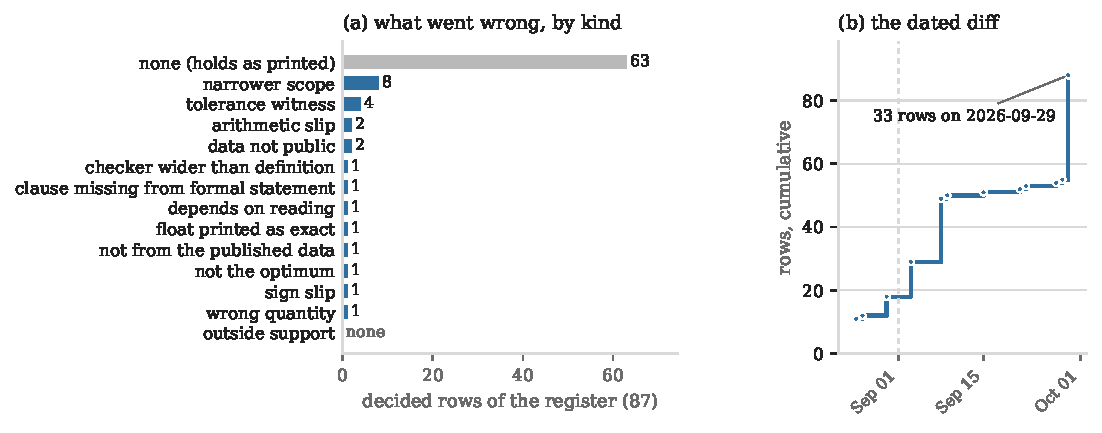
\includegraphics[width=\linewidth]{fig/register-kinds.pdf}
\caption{(a) The \RegDecided{} decided rows by defect kind; the vocabulary's kinds with no row are drawn empty. (b) The register as a dated diff: cumulative rows by the day a record first held them, with the month boundaries dashed. Both panels are drawn from \texttt{certs/claims-ledger.json}.}\label{fig:kinds}
\end{figure}

\section{Three worked examples}\label{sec:examples}

\subsection{A refutation and its witness}\label{sec:cstar}

Erd\H{o}s problem \#852 concerns a counting function whose conjectured asymptotic rests on two constants; both were posted to the problem thread on \CstarThreadDate{} as bare decimals, produced with a frontier model's help \cite{ErdosProblems}. The second, $C^*$, was printed to \CstarPublishedDigits{} significant digits, $\CstarPublished$.

The instrument encloses $C^*$ by a directed-rounding partial product over the \CstarPrimes{} odd primes below \CstarPrimeBound{} at \CstarBits{} bits, with the tail bounded by $\sum_{p>L}1/(p-1)^3\le1/(2(L-1)^2)$ and $\prod(1+a_p)\le e^S\le1+S+S^2$; the enclosure is the one in Theorem~\ref{thm:cstar}. The published decimal lies below it. That alone is a refutation, but it rests on the tail bound and on the rounding mode, and a reader who distrusts either should not have to. So the certificate also carries a witness that needs neither: the exact rational $N/D=\prod_{3\le p\le\CstarLimit}((p-1)^3+1)/(p-1)^3$, a strict lower bound of the full product because every further factor exceeds one, already satisfies $(N/D-1)/2>\CstarWindowNum/10^{\CstarWindowDen}$, the upper edge of the published claim's window under both the truncation and the rounding reading. That is the one integer inequality of Theorem~\ref{thm:cstar}, and a standard-library verifier (\texttt{\CstarVerifier}) re-decides it with no code from this repository.

The record also names the mechanism, which is the point of the example for the register. The published decimal equals the naive IEEE-754 double product of the defining formula: the factor $1+1/(p-1)^3$ rounds to exactly $1.0$ once $(p-1)^3\ge2^{53}$, that is for $p-1\ge\CstarThreshold$, so about \CstarVanish{} of the factors vanish and the floating-point product truncates itself near $p\sim2\cdot10^5$ whatever the loop bound. The register's kind for the row is \emph{float printed as exact}. The thread's other constant, $c_0=\CzeroPublished\ldots$, is correct as a rounding and is recorded so, with \CzeroDigits{} certified decimals beside it: a grammar that can say ``correct as a rounding'' keeps a refutation from reading as a judgement of the whole post.

\subsection{A repair}\label{sec:repair}

The optimisation-constants registry \cite{OptReg} (commit \SpRegistryCommit) marks bounds whose verification is at minimal levels with an asterisk; its row for the real sum--product exponent quotes, from a note of \SpNoteDate{} by \SpNoteAuthor{} written with a chat model \cite{Althoefer26}, the bound $C_{84b}\le1.999281$, that is $c\ge\SpQuotedC$, and marks it unverified. The note's own theorem claims only $c\ge\SpTheoremC$ and says that the optimised value suggested by the same calculation is about \SpQuotedC{}, with \SpTheoremC{} the safer constant to quote. The registry quoted the suggestion.

The instrument decided the note's chain: its seven numerical facts, each in interval arithmetic, and then the one question the registry row turns on --- whether any choice of the chain's free parameters reaches the quoted exponent (Table~\ref{tab:sp}). None does: the chain's ceiling is $c\le\SpCeiling$, below \SpQuotedC{}, and the note's own choice gives $c=\SpAtNote$. The row is therefore \textsc{repaired}: the claim as the registry prints it is refuted, and the object next to it --- the note's theorem, $c\ge\SpTheoremC$, given its cited inputs --- is certified. The kind is \emph{arithmetic slip}: a printed arithmetic step that does not hold, here the passage from a calculation to a constant the calculation cannot produce. What the row does not decide is the chain's inputs, which are a published paper's and a lemma's; Proposition~\ref{prop:repair} is conditional on them and says so.

\begin{table}[h]\centering\scriptsize
\begin{tabular}{@{}rp{0.62\linewidth}p{0.26\linewidth}@{}}\toprule
 & the check, as the record names it & what it found \\\midrule
\SpCheckRows
\bottomrule\end{tabular}
\caption{The \SpChecks{} checks of the C84b record, verbatim. The last is the one that repairs the row.}\label{tab:sp}
\end{table}

The same composition decides a different failure in the EinsteinArena table. A circle packing published as $\Sigma r=\EaCirclesPrinted$ has, in exact arithmetic on its own bytes, \EaCirclesOverlaps{} overlapping pairs and a bounding box over its limit --- all within the $10^{-9}$ slack the platform's verifier allowed when the packing was published (\EaCirclesPublished), a slack the platform removed on \EaCirclesSlackDropped; its live verifier, read on \EaRuleAsOf, rejects the file. Scaling every radius by the largest rational $\lambda$ that clears every pair and the box gives an exact witness of $\EaCirclesExact\ldots$, a deficit of \EaCirclesDeficit{} against the printed value; the printed digits are not the exact value's, and the row says which digit moved. The \EaOverlapRepairs{} minimum-overlap step functions whose sums miss $n/2$ by up to \EaOverlapMiss{} are repaired the same way, by a rescaling that moves each bound by at most \EaOverlapDeltaMax{}. In every repaired row the bound survives; what the repair records is that the bytes as published were not yet a witness, and by how much.

\subsection{A refusal, and what would decide it}\label{sec:refusal}

A published design table \cite{Bhaskaran23} prints annual-maximum $H_s$ fits --- four methods, \DtAreas{} South Atlantic lease areas, \DtDecided{} rows --- from a commercial hindcast (\DtPrivate) that cannot be re-run outside it. The claim is of the decidable kind: a fitted distribution either is or is not the likelihood's maximum on the series it was fitted to, and the project's return-level instrument decides that by a Krawczyk box on the score with the Hessian proved negative definite over it, as it has on the public benchmark buoys \cite{Haselsteiner21}. What is missing is the series.

The row is \textsc{needs data}, kind \emph{data not public}. It is not left empty. Against the nearest open-sea cells of the public hindcast the paper also names (\DtPublic), \DtKmMin{}--\DtKmMax{} km from the printed coordinates, with \DtYears{} calendar-year maxima each, the printed fits are \DtOff{} times off the certified maximum and once outside the record's support (Table~\ref{tab:dt}). The instrument reports these as the distance between two records --- two hindcasts at two points --- and refuses to call them errors in the table, because the verdict would depend on data the authors have and the instrument does not. What would decide the row is one file: the annual maxima the authors fitted at the five sites. With it, each printed row decides in minutes, as the printed fits of the contour benchmark's teams did.

\begin{table}[h]\centering\footnotesize
\begin{tabular}{@{}lrrrr@{}}\toprule
lease area & Gumbel, least squares & Gumbel, max.\ likelihood & Gumbel, moments & GEV, max.\ likelihood \\\midrule
\DtMatrixRows
\bottomrule\end{tabular}
\caption{The \DtDecided{} printed 100-year $H_s$ levels (m) against the certified fit's at the nearest public cell, as printed / certified. The differences, from \DtMinGap{} to \DtMaxGap{} m, measure two records' distance, not the table's correctness; a \textsc{needs data} row publishes them so the reader can see what the missing bytes would settle.}\label{tab:dt}
\end{table}

The precedent for this kind of row is in the kissing ledger \cite{Kissing}. On \KissNeedsFrom{} the headline \KissN{}-point configuration of one platform was not published; the row read \textsc{needs data} and named the bytes that would decide it. The platform published them on request on \KissBytes{}, \KissDays{} days later, and the row decided \textsc{certified} in \KissMs{} ms with \KissContacts{} exact contacts. \textsc{needs data} is the one verdict that can go to zero by the claimant's act, and the register is built so that the act is cheap.

\section{What the register measures}\label{sec:measures}

A register of self-chosen claims is not a sample of the field (\S\ref{sec:notclaimed}). What it measures is the \emph{kind} of thing that goes wrong, and the vocabulary was built for that: closed, each kind defined in one sentence, a new kind a decision about the world made in one place (Table~\ref{tab:kinds}).

\begin{table}[h]\centering\scriptsize
\begin{tabular}{@{}lp{0.52\linewidth}rr@{}}\toprule
kind & definition & rows & items \\\midrule
\KindRows
\bottomrule\end{tabular}
\caption{The closed vocabulary of \RegKinds{} kinds. Rows: register rows of that kind (an aggregate row by its most frequent defect; the queued row counts under none). Items: the same with the \RegAggregates{} aggregate rows opened, so that the \AggItems{} keys, contours, fits and sheet rows inside them are counted one by one.}\label{tab:kinds}
\end{table}

Four readings of the table are supported by the record.

\emph{Most claims hold.} \RegHolds{} of the \RegDecided{} decided rows name nothing wrong, \RegHoldsPct{}; the \RegTheorems{} rows that are theorems (\textsc{certified} or \textsc{refuted}) split \VCertified{} to \VRefuted{}. Inside the aggregates the proportion is higher still: of the GSM8K keys \cite{Cobbe21}, \GsAnnotExact{} of \GsAnnotations{} calculator annotations are exact (\GsAnnotRefused{} were refused) and \GsWrong{} printed prose steps of \GsItems{} keys do not hold; of the contour benchmark's \EcContours{} contours, \EcAgree{} of \EcComparisons{} printed exceedance counts agree with the exact count (\EcExact{} exactly) and \EcDisagree{} do not; of METR's \MeFits{} time-horizon fits \cite{Kwa25}, all are certified and the printed coefficients are the rounding of the certified optimum for \MeReproduced{} of \MeLive{} models. A register that led with its refutations would misreport its own content.

\emph{The most frequent defect is a statement about reach, not error.} \emph{Narrower scope} (\KNarrower{} rows) is the kind of all but one \textsc{partial} row (that one depends on a reading only its author can settle): a certified fragment beside a core --- an asymptotic reduction, an all-$m$ argument, a cited realisation theorem --- that is prose and was not touched. The six-lane audit of AI-assisted manuscripts is the clearest case (Table~\ref{tab:lanes}): \AiConfirmed{} of \AiLanes{} lanes certified and \AiPartial{} partial, and in all \AiLanes{} the computational fragment certified while the analytic core did not, because the core is not machine-checkable at any budget this project has.

\emph{The defects are the verifier's, not the mathematician's.} Of the \RegKindsUsed{} kinds that occur, the ones that name a wrong mathematical object are rare: one sign slip in a printed sheet, one float printed as exact, two arithmetic slips (one of them the \GsWrong{} GSM8K steps). The others describe the checking: witnesses that hold only within a verifier's tolerance (\KTolerance{} rows); a checker that accepts a pair if either of two one-sided tests passes where its definition needs both (\KChecker{} row, \S\ref{sec:hm}); a claim that holds under one of two definitions its own text gives (\KReading{} row); a printed number that is a correct answer to a different question (\KWrongQuantity{} row); printed numbers not what the published data give (\KNotFromData{} row); an optimiser's stop printed as the optimum (\KNotOptimum{} row); and data nobody outside can decide on (\KDataNotPublic{} rows). One kind occurred and has left the register: a clause in a paper's theorem that is absent from the formal statement that was proved. Its one row, OpenAI's Navier--Stokes certificate \cite{OpenAINS}, read \textsc{partial} from \NsPriorRecorded{} at the announced commit \NsCommit{}: \NsJobs{} modules built here with only the standard axioms, and the finite-energy clause of the paper's Theorem~1.1 not in the statement. The one upstream commit since, \NsHeadCommit{} of \NsHeadDate, proves that theorem with the clause; rebuilt here on the standard axioms, it moved the row to \textsc{certified} on \NsRecorded, with the \textsc{partial} kept as the row's history and the kind left with \KClause{} rows (Table~\ref{tab:kinds}). The defect was real at the commit the claim was announced on, and the register keeps both dates.

\emph{Who produced the bytes is not what this register measures.} By a coarse rule --- the claimant field names an AI system --- \AiRows{} decided rows are machine-produced and \OtherRows{} are not; \AiRowsDefects{} of the former and \OtherRowsDefects{} of the latter name a defect. The rule is a regular expression over a text field and the register was not sampled; the number is reported because a reader will ask. Here the machine-produced rows name a defect less often, but a coarse rule over an unsampled register supports no conclusion about either population.

\begin{table}[htb]\centering\scriptsize
\begin{tabular}{@{}llp{0.3\linewidth}rr@{}}\toprule
lane & verdict & scope & checks & controls \\\midrule
\LaneRows
\bottomrule\end{tabular}
\caption{The six-lane audit \cite{Ramsey}: six results produced with frontier-model help, re-verified from the manuscripts by verifiers that never executed the authors' code; \AiChecks{} named checks from the \AiChecksFrom{} lanes whose verifiers print a ledger, \AiMutations{} mutation controls, \AiSeconds{} s at every build. The lane pages say \textsc{confirmed} where the register says \textsc{certified}. A verifier that prints no per-check ledger is shown with a dash rather than an invented count.}\label{tab:lanes}
\end{table}

\subsection{The second refutation: a checker wider than its definition}\label{sec:hm}

HorizonMath \cite{Wang26} credits a frontier model with a certificate improving the Gupta--Ndiaye--Norin--Wei bound on diagonal Ramsey numbers \cite{GNNW24} from $\HmGnnw$ to $\HmC\ldots$, validated by the benchmark's own checker. The instrument re-derived the constant and then decided the one thing the checker had not: whether the certificate's pairs lie in the region $R$ that the paper's Theorem~14 requires. The pair at the point where the constant is read, $(X(1),Y(1))=(\HmXone,\HmYone)$, is outside $R$ --- Erd\H{o}s's 1947 bound at $\varepsilon=\HmGapE$, $p=\HmGapP$ exceeds the pair's rate by \HmGap{} --- and \HmOutside{} of the certificate's \HmPoints{} decided points are outside $R$, with \HmNotPlaced{} more not placed in $R$ by the bound the problem names. The cause is in the problem's own rule: it accepts every pair with $x\le e^{-U(1)}=\HmEU$ whatever $y$ is, asking one of the two inequalities membership needs; the benchmark's validator, at line \HmCheckerLine{}, takes a minimum where the definition takes a maximum, and with that one word changed it fails the certificate on its first interval. The row is \textsc{refuted}, kind \emph{checker wider than definition}; what is refuted is the certificate, not the inequality, and the scope sentence says so. The same benchmark's Kakeya construction is \textsc{certified} exactly: the union of its \HmKakeyaPieces{} pieces has area $\HmKakeyaNum/\HmKakeyaDen=\HmKakeyaDec\ldots$, below the baseline it claims to beat. The GNNW iteration that the paper itself prints as preliminary and unverified is certified too, by two independent implementations, with $c=\GnC\ldots$, of which the printed $3.78233$ is \GnPrintedIs{} \cite{Ramsey}.

\subsection{Refusals, by kind, each with its denominator}

\begin{table}[htb]\centering\scriptsize
\begin{tabular}{@{}lp{0.5\linewidth}rrl@{}}\toprule
kind & where & count & of & denominator \\\midrule
\RefusalRows
\bottomrule\end{tabular}
\caption{Every refusal on record, by kind, as the refusals page keeps them \cite{Refusals}: \RefKinds{} kinds, each a fraction of its own population, no total. The grader's refusal rate on submitted model proposals is \EvRefusalRate{} (\EvMalformed{} of \EvClaims{}; \EvCertified{} certified, \EvRejected{} refuted); the \EvDeclined{} replies in which the model declined and the \EvBudget{} cut off by the harness's own output cap are in neither numerator nor denominator.}\label{tab:refusals}
\end{table}

The refusal with the largest population is neither the instrument's nor the claimant's: \RefUndecided{} of \RefCells{} cells of two exhaustive parameter sweeps (\RefUndecidedPct{}) did not close at the budget, and are drawn on the atlas as holes rather than filled in by interpolation. A map with no holes drawn is a map that interpolated somewhere.

\section{Records re-certify}\label{sec:recert}

A method that decides other people's claims from their bytes must accept the same from others, and the register would be a one-way instrument if nothing ever ran in the other direction. One row has. The proof of the value of $\lambda(4)$ \cite{Lambda4} is a finite front: \LfGeneric{} generic collisions and \LfFamilies{} families, within which \LfClosed{} finite sets are decided by certificates against the target enclosure, with the extremizer $\{1,2,3,4\}$ skipped as the definitional witness \LfSkips{} times, once per finite part it lies on. The project's own audit of it (\LfDate) walked all \LfSets{} gcd-reduced $4$-sets with largest element at most \LfBox{} with code sharing nothing with the engine, re-certified \LfFinite{} finite-clause sets afresh and found \LfRefuters{} refuters.

On \LfOutsideDate{} an outside audit \cite{Lambda4Audit}, posted on the Erd\H{o}s problems issue for the problem, re-derived the cubic, the collisions and the families from the write-up with its own code, re-certified every finite case in interval arithmetic, and swept every gcd-reduced $4$-set with largest element at most \LfOutsideMax{} as a proof-independent control; $\{1,2,3,4\}$ was deepest and the nearest rival \LfRival{} at about \LfRivalValue{}. Its \LfFindings{} documentation findings --- a skip count the write-up had stated wrongly, a cone omitted from one family's listing, and a cubic described in the pull request to the problem's site as having a unique root where it has three real ones with $\lambda(4)$ the largest --- were folded into the write-up, and the skip count is now computed from the record so the build refuses if it moves. The audit's verdict was that nothing breaks; the register treats it as it treats a row it decided: a record, a date, a witness (the audit repository), and a defect kind for the write-up's prose rather than the theorem.

\section{What is not claimed}\label{sec:notclaimed}

\begin{itemize}\itemsep2pt
\item No theorem of anyone else's is proved or disproved here beyond its computational fragment. Where a row is \textsc{partial}, the analytic core was not audited, because it is not machine-checkable; confirming the identities a proof uses is not confirming the proof.
\item The register is not a sample. Every row is self-initiated and \RegSubmitted{} were submitted by others; the fraction of rows with a defect is a fact about this register and supports no estimate of an error rate in the field.
\item A refutation is of the object as printed. The HorizonMath row refutes a certificate, not the Ramsey inequality; the EinsteinArena repairs refute bytes as witnesses, not bounds; the C84b row refutes a quoted constant, not the note's theorem.
\item ``No shared code'' is independence from the claimant, not from the project's own past. Two instruments reuse the project's own code across a producer/checker line and are disclosed in the positioning note \cite{Positioning}; in one lane an author's script was read, not run, and the lane says so.
\item Several claims had already been checked by their authors, in two cases by an interval certificate the authors shipped; an independent reimplementation is not a first verification, and no row says it is.
\item Rows conditional on a cited argument are conditional: the C84b repair on the note's chain, the GNNW rows on the paper's Theorem~14, Lemma~15 and Theorem~1, five counterexample-library rows on the universal theorems or all-$m$ arguments their cases cite.
\item The register counts rows, not items. The \RegAggregates{} aggregate rows hold \AggItems{} items between them; a table that counted those as rows would be a bigger number and a smaller fact.
\item One erratum, found while writing this paper. The Ramanujan Machine audit holds \RmCertified{} certifications: \RmPrinted{} printed sheet rows, of which \RmSurvive{} survive and \RmRefuted{} is refuted as printed, plus \RmCorrections{} certified correction of the project's own, counted separately on the audit page \cite{Ramsey}. The register's row for it \RmErratum{} the correction among the printed rows (its text says \RmRegisterPrinted{} printed rows), against the project's own counting rule. Verdict, kind and every count above are unaffected; the sentence is to be fixed where the row is derived.
\end{itemize}

\section{Limits}\label{sec:limits}

The method's reach is the register's scope sentence: \RegScope{} The instrument cannot decide asymptotics, statements over infinite families with no finite reduction, or proofs whose content is prose; it refuses them, and a refusal says nothing about the claim. Within reach, cost is the limit that shows in the record: a sweep's undecided cells, a campaign's exhausted degree, a family still computing. The vocabulary of defect kinds is closed but not finished; it has \RegKinds{} entries after \RegRows{} rows and will be extended by the first claim that fits none, at which point the register refuses until the kind is decided. Dating by the first commit is exact for the record and late for the work. The register is one laboratory's, and the direction of \S\ref{sec:recert} has run once; that records re-certify is, so far, one row's worth of evidence. Finally, the discipline catches bugs by running the machine, not by reading it (Table~\ref{tab:bugs}), which is a reason to trust the controls and not a reason to trust the code.

\cmrepro{\sloppy The register is \path{certs/claims-ledger.json}, written by \texttt{node} \path{tools/run-claims-ledger.js} from the records it names in each row's \texttt{decidedFrom}; the claims desk, the refusals page and the monthly ledger are built from it by the three \path{tools/build-report-*.js} builders of those names. The three worked examples re-run from their records: \texttt{python3} \path{tools/verify_erdos852.py} decides Theorem~\ref{thm:cstar} with the Python standard library alone; \texttt{python3} \path{tools/run-sumproduct-ledger.py} \texttt{--check} and \path{instruments/sumproduct/battery.py} re-derive Proposition~\ref{prop:repair}; the design-table audit is \path{certs/design-table-audit.json} with the printed-fit decider \path{playground/return-level-check/printed.js}. The in-house $\lambda(4)$ audit is \path{tools/audit-lambda4.js} (record \path{certs/lambda4-audit.json}); the outside audit is at \url{\LfOutsideUrl}. The macros of this document are written by \path{tools/paper-numbers/register.js} from the records named in its header, and the figure by \path{tools/paper-numbers/register-fig.py}; the tool refuses when a record no longer says what a sentence needs. Built at git \RepoCommit{} from the register of \RegDate{} (git \RegGit{}).}

\begin{thebibliography}{99}\scriptsize\setlength{\itemsep}{1pt}
\bibitem{Novikov25} A.~Novikov, N.~V\~u, M.~Eisenberger et al., AlphaEvolve: a coding agent for scientific and algorithmic discovery, arXiv:2506.13131 (2025).
\bibitem{Georgiev25} B.~Georgiev, J.~G\'omez-Serrano, T.~Tao, A.~Z.~Wagner, Mathematical exploration and discovery at scale, arXiv:2511.02864 (2025).
\bibitem{Fawzi22} A.~Fawzi et al., Discovering faster matrix multiplication algorithms with reinforcement learning, Nature 610 (2022), 47--53.
\bibitem{Strassen69} V.~Strassen, Gaussian elimination is not optimal, Numer.\ Math.\ 13 (1969), 354--356.
\bibitem{Bianchi26} F.~Bianchi, Y.~Kwon, A.~Pappu, J.~Zou, Harnessing the collective intelligence of AI agents in the wild for new discoveries, arXiv:2606.10402 (2026).
\bibitem{Chung26} S.~Chung, W.~Du, W.~J.~Wesley et al., Autonomous mathematical discovery in an open-world multi-agent environment, arXiv:2608.23691 (2026).
\bibitem{Yuksekgonul26} M.~Yuksekgonul, D.~Koceja, X.~Li et al., Learning to discover at test time, arXiv:2601.16175 (2026).
\bibitem{Haugland16} J.~K.~Haugland, The minimum overlap problem revisited, arXiv:1609.08000 (2016).
\bibitem{Ganzhinov22} M.~Ganzhinov, Highly symmetric lines, arXiv:2207.08266 (2022).
\bibitem{Wang26} E.~Y.~Wang, S.~R.~Motwani, J.~V.~Roggeveen et al., Measuring progress in reasoning toward mathematical discovery with automatic verification, arXiv:2603.15617 (2026).
\bibitem{Sra26} S.~Sra, GPT, the counterexample machine, arXiv:2608.29595 (2026); library at \url{https://github.com/suvrit/count-ex-machina}, commit \CxCommit{} as recorded in \texttt{certs/countex-ledger.json}.
\bibitem{GNNW24} P.~Gupta, N.~Ndiaye, S.~Norin, L.~Wei, Optimizing the CGMS upper bound on Ramsey numbers, arXiv:2407.19026 (2024).
\bibitem{Gao26} S.~Gao, Counterexamples to the Jacobian conjecture in dimensions greater than two, arXiv:2608.00222 (2026).
\bibitem{CHV26} \'A.~Casta\~neda, G.~Honorato, F.~Valenzuela-Henr\'iquez, The weak Markus--Yamabe conjecture fails in dimension 14, arXiv:2608.05392 (2026).
\bibitem{Cobbe21} K.~Cobbe, V.~Kosaraju, M.~Bavarian et al., Training verifiers to solve math word problems, arXiv:2110.14168 (2021).
\bibitem{Kwa25} T.~Kwa, B.~West, J.~Becker et al., Measuring AI ability to complete long software tasks, arXiv:2503.14499 (2025).
\bibitem{Haselsteiner21} A.~F.~Haselsteiner et al., A benchmarking exercise for environmental contours, Ocean Engineering 236 (2021), 109504.
\bibitem{Bhaskaran23} S.~K.~Bhaskaran, A.~S.~Verma, A.~J.~Goupee, S.~Bhattacharya, A.~R.~Nejad, W.~Shi, Comparison of extreme wind and waves using different statistical methods in 40 offshore wind energy lease areas worldwide, Energies 16 (2023), 6935, doi:\DtDoi.
\bibitem{OptReg} The optimization-problems registry, \url{https://github.com/teorth/optimizationproblems}, commit \OcRegistryCommit{} as recorded in \texttt{certs/sumdiff-ledger.json}; its README: ``\OcStarNote''.
\bibitem{Althoefer26} \SpNoteAuthor, \SpNoteTitle, note of \SpNoteDate, \url{https://althofer.de/improved_constant_052.tex}, pinned by sha256 in \texttt{certs/sumproduct-ledger.json}.
\bibitem{ErdosProblems} Erd\H{o}s problem \#852 and its thread, \url{https://www.erdosproblems.com/852}, pinned by sha256 in \texttt{certs/erdos852-certificate.json}; report \url{https://carlostoledo.co/reports/erdos852.html}.
\bibitem{OpenAINS} OpenAI, NavierStokesAndEuler, \url{https://github.com/openai/NavierStokesAndEuler}, commit \NsCommit{} as recorded in \texttt{corpus/navier-stokes/build.json} and commit \NsHeadCommit{} as recorded in \texttt{corpus/navier-stokes/upstream-f9e8bc5b.json}; report \url{https://carlostoledo.co/reports/navier-stokes.html}.
\bibitem{MC100} One hundred machine claims, pre-registered \McRegistered{} before any was decided, \texttt{corpus/machine-claims-100.json}, decided pool by pool into \texttt{certs/mc100-*.json}, \url{https://github.com/carlostoledo1891/cert-machine}.
\bibitem{Xin26} E.~Xin, Where the verifier fails: a category-level audit of reward signals in RLVR, arXiv:2609.01354 (2026).
\bibitem{MKC09} R.~E.~Moore, R.~B.~Kearfott, M.~J.~Cloud, Introduction to Interval Analysis, SIAM, Philadelphia, 2009.
\bibitem{Tucker11} W.~Tucker, Validated Numerics: A Short Introduction to Rigorous Computations, Princeton University Press, 2011.
\bibitem{Hales17} T.~Hales et al., A formal proof of the Kepler conjecture, Forum Math.\ Pi 5 (2017), e2.
\bibitem{Lambda4} C.~Toledo, The value of $\lambda(4)$: a machine-derived proof completing Mercer's Section-5 program, \url{https://carlostoledo.co/reports/lambda4.html}, doi:10.5281/zenodo.22225861 (2026).
\bibitem{Lambda4Audit} rainrzk, erdos510-lambda4-audit, \url{\LfOutsideUrl}, posted on \url{https://github.com/teorth/erdosproblems/issues/\LfIssue} (\LfOutsideDate).
\bibitem{Kissing} C.~Toledo, Two platforms, one configuration: independent exact certification of the dimension-eleven kissing records, \url{https://carlostoledo.co/reports/kissing.html} (2026).
\bibitem{Erdos1} C.~Toledo, Explicit sum-distinct sets below Bohman's constant: the Erd\H{o}s problem \#1 disproof made effective, certificates at doi:10.5281/zenodo.22800699 (2026).
\bibitem{Positioning} Positioning: the decisions, \texttt{notes/positioning-decisions-2026-09-03.md}, \url{https://github.com/carlostoledo1891/cert-machine}.
\bibitem{MethodsNote} None by reading code: the methods note, \url{https://carlostoledo.co/reports/methods-note.html}.
\bibitem{Refusals} What the machine would not decide, \url{https://carlostoledo.co/reports/refusals.html}; the claims desk, \url{https://carlostoledo.co/reports/claims.html}.
\bibitem{Monthly} Decided, September 2026, \url{https://carlostoledo.co/reports/decided-2026-09.html}.
\bibitem{Ramsey} Report pages under \url{https://carlostoledo.co/reports/}: the six-lane audit, \texttt{ai-claims-audit.html} (one page per lane, \texttt{claim-\textit{id}.html}); \texttt{diagonal-ramsey.html}; \texttt{horizonmath.html}; the Ramanujan Machine's sheets, \texttt{rm-audit.html}.
\end{thebibliography}

\end{document}
